\documentclass[a4paper]{article}

%% Language and font encodings
\usepackage[english]{babel}
\usepackage[utf8x]{inputenc}
\usepackage[T1]{fontenc}
\usepackage{caption}

%% Sets page size and margins
\usepackage[a4paper,top=3cm,bottom=2cm,left=3cm,right=3cm,marginparwidth=1.75cm]{geometry}

%% Useful packages
\usepackage{amsmath}
\usepackage{amsfonts}

\usepackage{graphicx}
\usepackage{tikz}
\usetikzlibrary{arrows.meta}

\usepackage[colorinlistoftodos]{todonotes}
\usepackage[colorlinks=true, allcolors=blue]{hyperref}

\usepackage{color}
\usepackage{url}

%% display solutions or not
\newif\ifsol
\soltrue % comment out to hide solutions

%% todo tracker -- overleaf v2 has better one it uses but will default to this if compiled on something that doesn't have built-in todo
%\newcommand{\todo}[1]{\textbf{\textcolor{red}{#1}}}

\title{Section 6: Reinforcement Learning}
\author{CS 182 - Artificial Intelligence}
\date{}

\begin{document}
\maketitle

\noindent We use \textbf{Reinforcement Learning (RL)} when we have a Markov Decision Process (MDP) for which we know: 
\begin{itemize}
    \item $S$: set of states
    \item $A$: set of actions (for any given state)
    \item $s_0$: start state
    \item $s_g$: goal state (or set of goal states)
\end{itemize}
but do not know:
\begin{itemize}
    \item $T : S \times A \to S$: transition map (or model)
    \item $R : S \times A \to \mathbb{R}$: reward function
\end{itemize}
The goal of reinforcement learning is to learn a \textbf{policy} $\pi: S \to A$ which returns the best action for any given state in the problem. In the process of looking for the policy, RL algorithms often calculate:
\begin{itemize}
    \item $V : S \to \mathbb{R}$: \textbf{value function}, which stores the utility of every state
    \item $Q : S \times A \to \mathbb{R}$: \textbf{Q-value function}, which stores the value of every (state, action) pair \\
\end{itemize}

\noindent In \textbf{Passive Reinforcement Learning}, an agent has a fixed policy, and learns about the environment while executing that policy. In lecture, we discussed two algorithms:
\begin{enumerate}
    \item \textbf{Direct evaluation} runs many "experiments", or "simulations", resulting from following a given policy $\pi$, and keeps track of the total discounted rewards of the visited states. Afterwards, the reward instances for each state are averaged to determine the state's value. This could be written as
    \[
    V(s) = \frac{1}{n} \sum_i (R(s_i) + \gamma R(s_i') + \gamma^2 R(s_i'') + ...)
    \]
    where $s_i$, $s_i'$, $s_i''$, $\dots$, are the states visited in the $i$th simulation. Direct evaluation can also be referred to as a \textbf{Monte Carlo} approach, since it depends on averaging over many randomized simulations or samples.
    \item \textbf{Temporal difference learning} iteratively runs experiments following a given policy. With each transition, a sample-based Bellman update is made to the value of the visited state (both equations are computing the same thing):
    \[
    V^{\pi}(s) \leftarrow V^{\pi}(s) + \alpha [R(s, \pi(s), s') + \gamma V^{\pi}(s') - V^{\pi}(s)]
    \]
    \[
    V^{\pi}(s) \leftarrow (1- \alpha) V^{\pi}(s) + \alpha [R(s, \pi(s), s') + \gamma V^{\pi}(s')]
    \]
    We can think of this algorithm can be thought of as sample-based policy evaluation. Remember policy evaluation was:
    $$V^{\pi}(s) \leftarrow \sum_{s'} T(s, \pi_k(s), s') [R(s,\pi(s),s') + \gamma V^{\pi}(s')]$$
    In Q-learning we are still executing some policy $\pi$ we just don't know what the transition model is and thus can't compute all of the possible transitions to sum over. Instead we are simply computing one of the values in the sum and making a weighted update of our current value to incorporate the new information.
\end{enumerate}

\noindent In \textbf{Active Reinforcement Learning}, and agent chooses actions and tries to find an optimal policy while learning about the environment. The primary algorithm used in active RL is \textbf{Q-learning}. Similarly to TD learning, Q-learning makes sample-based Bellman updates, but to Q-values instead of values:
\[
Q(s, a) \leftarrow Q(s, a) + \alpha [R(s, a, s') + \gamma \max_{a'} Q(s', a') - Q(s, a)]
\]
\[
Q(s, a) \leftarrow (1 - \alpha) Q(s, a) + \alpha [R(s, a, s') + \gamma \max_{a'} Q(s', a')]
\]
Since we are learning Q-values and not values we can extract the current estimate of the optimal policy by doing a one-step argmaximization over the Q-value immediately at any time: \\
\[
\pi(s) = arg\max_{a} Q(s,a)
\]

\noindent Some algorithmic details and variations:
\begin{enumerate}
    \item In active algorithms, we must choose actions to take from states. One approach is \textbf{$\epsilon$-greedy action selection}: with (small) probability $\epsilon$, actions are chosen randomly; with (large) probability $1 - \epsilon$, we choose the current optimal action. This encourages exploration of the state space and is generally helpful in practice. Note that this is called off-policy learning as we learn the exact Q-values but execute with a different policy, the $\epsilon$-greedy policy.
    \item How can we evaluate the choice of parameters or exploration functions in Q-learning? One approach is to measure \textbf{regret} -- the difference between expected rewards and final optimal rewards.
    \item In linear \textbf{approximate} (or \textbf{feature based}) \textbf{Q-learning} we approximate the Q-function with a set of functions which are intended to represent higher-level features of the state space: 
    \[
    Q(s,a) = w_1 f_1(s,a) + w_2 f_2(s,a) + \dots + w_m f_m(s,a)
    \]
    For example, for PACMAN they could be the number of ghosts, the distance to the nearest ghost, the distance to the nearest food, etc. The advantage here is that we simply need to learn the correct weights, and thus we have fewer parameters to learn than in standard Q-learning, where we have to learn a table of Q-values for every single state-action pair. The disadvantage is that the quality of the Q-values is highly dependent on the quality of the functions. The update of the weights based on new information is:
    \[
    w_i \leftarrow w_i + \alpha f_i(s,a) [R(s, a, s') + \gamma \max_{a'} Q(s', a') - Q(s, a)]
    \]
    
\end{enumerate}

\noindent Algorithmic parameters:
\begin{itemize}
    \item $\alpha$: learning rate (determines the integration of new information into current estimates)
    \item $\gamma$: discount rate (determines how quickly rewards decay with time)
\end{itemize}

\newpage
\section*{Practice Problems}
\begin{enumerate}
    \item Suppose we are Q-learning with $\epsilon$-greedy action selection, starting with $\epsilon = 0.2$. When is it a good idea to...
    \begin{itemize}
        \item keep $\epsilon$ constant over time?
        \item decrease $\epsilon$ to 0 over time?
        \item increase $\epsilon$ over time?
    \end{itemize}
    
    \ifsol
        \textcolor{blue}{It is generally good to decrease $\epsilon$ to 0 with time, especially when using on-policy learning methods. The reason is that as the agent learns the actual optimal policy for the world, it should switch from a mix of exploration and exploitation to mostly exploitation. However, if the world is changing, we may leave $\epsilon$ high such that the agent would continue to explore. It never makes sense to continuously increase $\epsilon$, as this counteract convergence.}
    \else
        \vspace{7em}
    \fi 
    
    \item Suppose we are Q-learning. When is it a good idea to...
    \begin{itemize}
        \item set $\alpha = 0$?
        \item set $\alpha = 1$?
        \item set $\alpha = 0.2$ and decrease it to 0 over time?
    \end{itemize}
    
    \ifsol
        \textcolor{blue}{If the learning rate $\alpha$ is set to 0, we will not make any updates to the value function, so this is never a good idea. When $\alpha$ is set to 1, we will be fully overriding prior value estimates with the new update. While this is generally undesirable, it is actually optimal for a fully deterministic MDP. The third option -- setting alpha to a low value and decreasing it over time -- is the most reasonable approach.}
    \else
        \vspace{7em}
    \fi 
    
    \item What would the returned value assignments be for Direct Evaluation over a deterministic MDP? Can you find a simple upper bound on the number of experiments that need to be run by the algorithm for the value function to converge? What if the MDP is not deterministic?
    
    \ifsol
        \textcolor{blue}{If the MDP is deterministic, Direct Evaluation would assign the exact value of every visited state under the given policy, so the number of necessary experiments would be no larger than the total number of start states. If the MDP is not deterministic, we do not have this guarantee, since separate experiments would have different returns.}
    \else
        \vspace{7em}
    \fi 
    
    \item When using features to represent the $Q$-function, is it guaranteed that the feature-based $Q$-learning finds the same optimal $Q^∗$ as would be found when using a tabular representation for the $Q$-function?
    
    \ifsol
        \textcolor{blue}{No -- the optimal Q-function $Q∗$ would depend on the choice of features. Even if the choice of features was fully informed, it may not be possible to represent the optimal $Q^*$ with a (linear) weighted combination of features.}
    \else
        \vspace{7em}
    \fi
    
    \item Why is temporal difference (TD) learning of Q-values (Q-learning) superior to TD learning of values?
    
    \ifsol
        \textcolor{blue}{If only values are found, it is difficult to extract a policy -- this would require knowing or calculating the transition function. If Q-values are found, the policy can be easily computed by $\pi(s) = \text{argmax}_a \; Q(s, a)$.}
    \else
        \vspace{7em}
    \fi
    
    \newpage
    \item Recall a problem from last week's section: Consider an MDP having three states, (1, 2, 3), where State 3 is a terminal state. In States 1 and 2, there are two possible actions: $A$ and $B$. Unlike last week, we no longer know the rewards or transition model ahead of time. \\
    
    Suppose we decide to run Q-learning on this problem with $\alpha = 0.2$ and a 0.9 discount ($\gamma = 0.9$). All Q-values are initialized to 0. While running one episode/simulation within the algorithm, we get the following $(s, a, s', r)$ samples (in order): \\
    
    (State 1, Action B, State 1, reward = -1) \\
    (State 1, Action A, State 1, reward = -1) \\
    (State 1, Action A, State 2, reward = -2) \\
    (State 2, Action B, State 2, reward = -2) \\
    (State 2, Action B, State 3, reward = 0) \\
    
    Run Q-learning based on these samples. How are the Q-values updated? \\
    \ifsol
        \textcolor{blue}{
    Initialization:
    \begin{center}
    \begin{tabular}{ |c|c|c| } 
     \hline
             & Action A & Action B \\ 
     State 1 & 0 & 0 \\ 
     State 2 & 0 & 0 \\ 
     State 3 & 0 & 0 \\ 
     \hline
    \end{tabular}
    \end{center}
    (State 1, Action B, State 1, reward = -1)  $\rightarrow$  (0.8 * 0 + 0.2 (-1 + 0.9 max(0, 0)) = -0.2)
    \begin{center}
    \begin{tabular}{ |c|c|c| } 
     \hline
             & Action A & Action B \\ 
     State 1 & 0 & -0.2 \\ 
     State 2 & 0 & 0 \\ 
     State 3 & 0 & 0 \\ 
     \hline
    \end{tabular}
    \end{center}
    (State 1, Action A, State 1, reward = -1)  $\rightarrow$  (0.8 * 0 + 0.2 (-1 + 0.9 max(0, -0.2)) = -0.2)
    \begin{center}
    \begin{tabular}{ |c|c|c| } 
     \hline
             & Action A & Action B \\ 
     State 1 & -0.2 & -0.2 \\ 
     State 2 & 0 & 0 \\ 
     State 3 & 0 & 0 \\ 
     \hline
    \end{tabular}
    \end{center}
    (State 1, Action A, State 2, reward = -2)  $\rightarrow$  (0.8 * (-0.2) + 0.2 (-2 + 0.9 max(0, 0)) = -0.56)
    \begin{center}
    \begin{tabular}{ |c|c|c| } 
     \hline
             & Action A & Action B \\ 
     State 1 & -0.56 & -0.2 \\ 
     State 2 & 0 & 0 \\ 
     State 3 & 0 & 0 \\ 
     \hline
    \end{tabular}
    \end{center}
    (State 2, Action B, State 2, reward = -2)  $\rightarrow$  (0.8 * 0 + 0.2 (-2 + 0.9 max(0, 0)) = -0.4)
    \begin{center}
    \begin{tabular}{ |c|c|c| } 
     \hline
             & Action A & Action B \\ 
     State 1 & -0.56 & -0.2 \\ 
     State 2 & 0 & -0.4 \\ 
     State 3 & 0 & 0 \\ 
     \hline
    \end{tabular}
    \end{center}
    (State 2, Action B, State 3, reward = 0)  $\rightarrow$  (0.8 * (-0.4) + 0.2 (0 + 0.9 max(0, 0)) = -0.32)
    \begin{center}
    \begin{tabular}{ |c|c|c| } 
     \hline
             & Action A & Action B \\ 
     State 1 & -0.56 & -0.2 \\ 
     State 2 & 0 & -0.32 \\ 
     State 3 & 0 & 0 \\ 
     \hline
    \end{tabular}
    \end{center}
    }
    \else
        \vspace{28em}
    \fi
    
    How would the solution be different if we chose all actions following the optimal policy? \\
    \ifsol
        \textcolor{blue}{At every step, the next chosen action (from a given state) will be the one corresponding to the largest current Q-values of that state. In the samples given above, all actions follow the current optimal policy except the last sample, where action A would have been taken instead of Action B, since $Q(\text{State 2}, \text{Action A}) > Q(\text{State 2}, \text{Action B})$.}
    \else
        \vspace{7em}
    \fi
    \newpage
    \item Consider the Pacman-inspired game board below. Suppose that every action has a 80\% chance of moving in the desired direction, and a 10\% chance of moving in each of two perpendicular directions (though we only learn this transition function by executing actions in the world). The lower left-hand square is numbered (0, 0), the start square is (3, 0), and the goal square is (0, 6). The goal of this game is for Pacman to navigate to the exit (reward of 100) without touching the dangerous explosion square at (1, 4), which terminates the game with a reward of $-100$. Pacman cannot cross the thick wall in the middle of the board; an action causing a wall collision would make Pacman stay in place.
    
    \begin{center}
    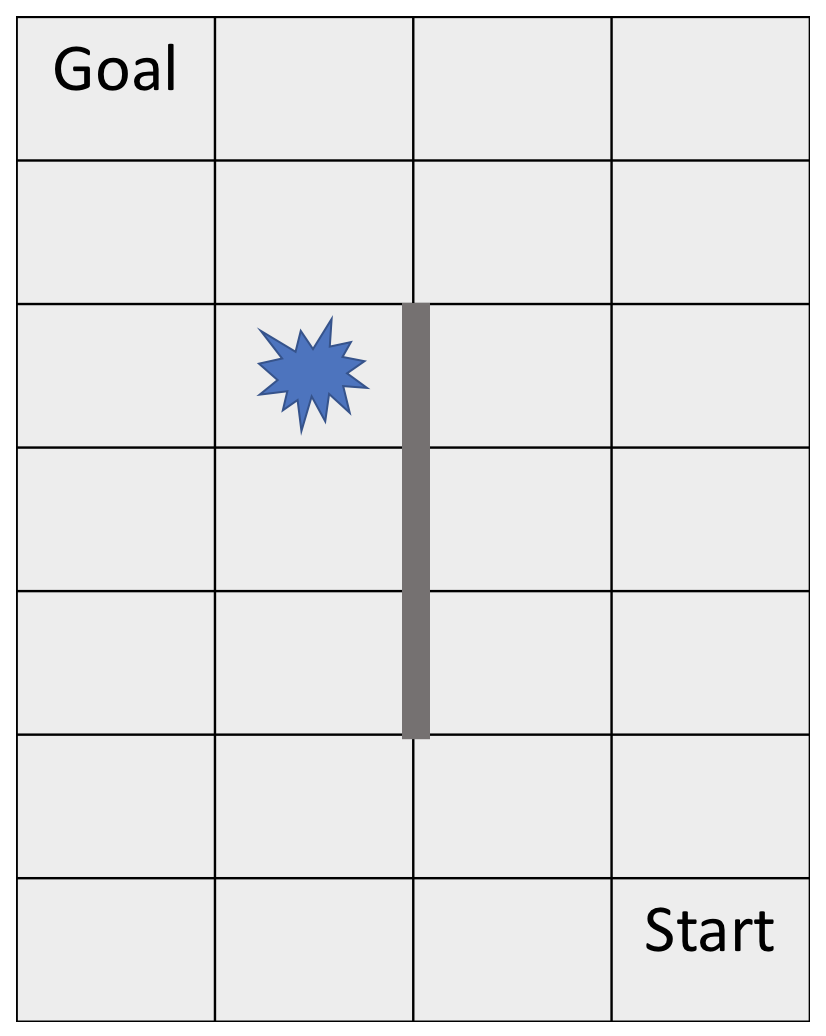
\includegraphics[scale=0.25]{grid.png}
    \end{center}
    
    Let's say we choose to solve this problem with feature-based Q-learning, with the features: \\
    $f_1 =$ the Manhattan distance to the goal \\
    $f_2 =$ 0 or 1 indicating whether the explosion square is in 1-square radius of Pacman.
    \begin{enumerate}
        \item Which gameboard squares will be equivalent to the state defined by ($f_1 = 4$, $f_2 = 1$)? \\
        \ifsol
            \textcolor{blue}{Squares (1, 3) and (2, 4) both have a Manhattan distance of $4$ to the goal, and are one square away from the square $(1, 4)$.}
        \else
            \vspace{5em}
        \fi
        
        \item What are the advantages and disadvantages of using this feature representation? \\
        \ifsol
            \textcolor{blue}{The advantage of a feature representation is that it decreases the number of states needed for the problem, so each transition informs a greater number of (grid) state values. The downside is that features may not capture important information. In this problem, if the explosion square is nearby but behind a wall, it does not pose a threat; but the feature representation equates this situation to one where there is a dangerous square and no wall.}
        \else
            \vspace{5em}
        \fi
    \end{enumerate}
\end{enumerate}


\end{document}